\documentclass[runningheads]{llncs}

\usepackage{appendix}
%\usepackage{lipsum}
\usepackage{graphicx}
\usepackage[hidelinks]{hyperref}
\usepackage{pgfgantt}
\usepackage{adjustbox}
\usepackage{pifont}
\usepackage{mcite}

% Copyright 2017 Sergei Tikhomirov, MIT License
% https://github.com/s-tikhomirov/solidity-latex-highlighting/

\usepackage{listings, xcolor}
\definecolor{verylightgray}{rgb}{.97,.97,.97}

\lstdefinelanguage{Solidity}{
	keywords=[1]{anonymous, assembly, assert, balance, break, call, callcode, case, catch, class, constant, continue, constructor, contract, debugger, default, delegatecall, delete, do, else, emit, event, experimental, export, external, false, finally, for, function, gas, if, implements, import, in, indexed, instanceof, interface, internal, is, length, library, log0, log1, log2, log3, log4, memory, modifier, new, payable, pragma, private, protected, public, pure, push, require, return, returns, revert, selfdestruct, send, solidity, storage, struct, suicide, super, switch, then, this, throw, transfer, true, try, typeof, using, value, view, while, with, addmod, ecrecover, keccak256, mulmod, ripemd160, sha256, sha3}, % generic keywords including crypto operations
	keywordstyle=[1]\color{blue}\bfseries,
	keywords=[2]{address, bool, byte, bytes, bytes1, bytes2, bytes3, bytes4, bytes5, bytes6, bytes7, bytes8, bytes9, bytes10, bytes11, bytes12, bytes13, bytes14, bytes15, bytes16, bytes17, bytes18, bytes19, bytes20, bytes21, bytes22, bytes23, bytes24, bytes25, bytes26, bytes27, bytes28, bytes29, bytes30, bytes31, bytes32, enum, int, int8, int16, int24, int32, int40, int48, int56, int64, int72, int80, int88, int96, int104, int112, int120, int128, int136, int144, int152, int160, int168, int176, int184, int192, int200, int208, int216, int224, int232, int240, int248, int256, mapping, string, uint, uint8, uint16, uint24, uint32, uint40, uint48, uint56, uint64, uint72, uint80, uint88, uint96, uint104, uint112, uint120, uint128, uint136, uint144, uint152, uint160, uint168, uint176, uint184, uint192, uint200, uint208, uint216, uint224, uint232, uint240, uint248, uint256, var, void, ether, finney, szabo, wei, days, hours, minutes, seconds, weeks, years},	% types; money and time units
	keywordstyle=[2]\color{teal}\bfseries,
	keywords=[3]{block, blockhash, coinbase, difficulty, gaslimit, number, timestamp, msg, data, gas, sender, sig, value, now, tx, gasprice, origin},	% environment variables
	keywordstyle=[3]\color{violet}\bfseries,
	identifierstyle=\color{black},
	sensitive=false,
	comment=[l]{//},
	morecomment=[s]{/*}{*/},
	commentstyle=\color{gray}\ttfamily,
	stringstyle=\color{red}\ttfamily,
	morestring=[b]',
	morestring=[b]"
}

\lstset{
	language=Solidity,
	backgroundcolor=\color{verylightgray},
	extendedchars=true,
	%basicstyle=\footnotesize\ttfamily,
	basicstyle=\fontsize{7}{9}\selectfont\ttfamily,
	showstringspaces=false,
	showspaces=false,
	numbers=left,
	numberstyle=\tiny,
	numbersep=9pt,
	tabsize=2,
	breaklines=true,
	showtabs=false,
	captionpos=b
}

\graphicspath{ {./figures/} }

% remove underfull \hbox log entries from bibliography
%\apptocmd{\sloppy}{\hbadness 10000\relax}{}{}

% hide default TOC heading
\renewcommand\contentsname{\vspace*{-30pt}}
%\renewcommand\UrlFont{\color{blue}\rmfamily}
\renewcommand{\figurename}{Figure}

% set how many levels of headings show up in table of contents
\setcounter{tocdepth}{3}
\setcounter{secnumdepth}{3}

\begin{document}

\title{Smart Contract Migration Across Heterogeneous Blockchains}
\author{Tiago Domingues\\\email{tiagofsdomingues@tecnico.ulisboa.pt}}
\authorrunning{Tiago Domingues}
\institute{Instituto Superior Técnico}

% omit page numbering
\pagenumbering{gobble}

% hack to omit title from table of contents (part 1/2)
\let\oldaddcontentsline\addcontentsline
\def\addcontentsline#1#2#3{}

\maketitle

% add date
\noindent \makebox[\linewidth]{\small January 2022}

% hack to omit title from table of contents (part 2/2)
\def\addcontentsline#1#2#3{\oldaddcontentsline{#1}{#2}{#3}}

\begin{abstract}
Since the emergence of Bitcoin over a decade ago, blockchain technology has been maturing at an unprecedented rate. The success of Ethereum allowed numerous possibilities and new blockchains with smart contract functionalities started to emerge. These new systems often present different trade-offs between decentralization, scalability and security. Having several blockchains in the ecosystem gives developers the liberty to choose which platform best suits their use-case and their application, depending on their requirements and the type of users they want to target. 

Since there are plenty alternatives for users and developers to choose from, interoperability and migration have become outstanding subjects in blockchain technology. There is an increasing need to allow users and applications to easily move across chains and take advantage of what these platforms have to offer. Therefore, systems that enable interoperability between blockchains and allow smart contracts to be migrated are required to fulfill the needs of the industry and to keep it moving forward.

This document proposes a tool to migrate smart contracts between heterogeneous blockchains. More precisely, it proposes an extension to an existing tool called \textit{Osprey}, that allows the translation of Solidity smart contracts to Hyperledger Fabric chaincode written in Typescript. The main goal is to add support to the translation of Typescript chaincode to Solidity, making \textit{Osprey} a full two-way migrating tool.

\keywords{Blockchain Interoperability \and Migration \and Translation \and Smart Contracts \and Ethereum \and Solidity \and Hyperledger Fabric \and Chaincode.}
\end{abstract}

% hack to change formatting of TOC heading to match formatting of section heading
\newpage

%----------------------------------------------------------------------------- 
\section*{Table of Contents}
{\let\clearpage\relax \tableofcontents}
\newpage

% start page numbering
\pagenumbering{arabic}


%----------------------------------------------------------------------------- 
\section{Introduction} \label{intro}

Since the emergence of Bitcoin \cite{nakamoto_2008} over a decade ago, blockchain technology has been maturing at an unprecedented rate. What was originally designed as a peer-to-peer electronic cash system that made radical developments in money and currency as we knew it, rapidly evolved into a more complex network of decentralized applications, with the launch of Ethereum \cite{buterin_2014}.

Ethereum was the first blockchain to provide the ability to use a Turing-complete programming language to write what is called a smart contract. As per Buterin's description, these contracts ``can be used to encode arbitrary state transition functions" \cite{buterin_2014}. Smart contracts drew attention from several fields (audits, education, finance, health care, insurance, etc.) and enabled a meaningful amount of systems and applications never imagined before (decentralized exchanges and liquidity providing, decentralized borrowing and lending, decentralized derivatives, DAOs, NFTs, etc.).

The success of Ethereum allowed numerous possibilities and, therefore, new blockchains with smart contract functionalities started to emerge. These new blockchains often present different trade-offs between decentralization, scalability and security, also know as The Blockchain Trilemma \cite{certik_2019}, termed by Vitalik Buterin. Having several blockchains gives developers the liberty to choose which platform best suits their use-case and their application, depending on their requirements and their target users. 

%trilemma figure
\begin{figure}
  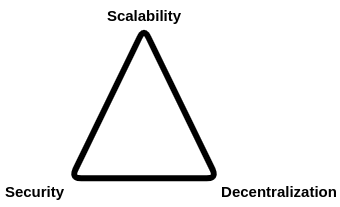
\includegraphics[scale=0.6]{trilemma.png}
  \centering
  \caption{The Blockchain Trilemma \protect\cite{certik_2019}}
  \label{fig:trilemma}
\end{figure}

Nowadays, Ethereum is by far the most widely used smart contract blockchain, but many others have been gaining a lot of traction and adoption by both developers and users. Some blockchains adopted the Ethereum Virtual Machine (EVM) \cite{buterin_2014} and opted to make more relevant changes on the consensus mechanism layer, such as Avalanche \cite{sekniqi_laine_buttolph_sirer_2020}, Binance Smart Chain \cite{binance_2020}, Fantom \cite{choi_park_nguyen_cronje_2018}, Harmony \cite{harmony}, among others. Alternatively, some blockchains have a whole new approach and decided not to reuse the EVM, such as Cardano \cite{cardano}, Cosmos \cite{cosmos}, Polkadot \cite{wood} and Solana \cite{yakovenko}.

The first type of platforms is very close to Ethereum in the sense that any Solidity smart contract deployed on the Ethereum blockchain can be easily deployed on any of these blockchains with few to zero changes, since the EVM is being used. Therefore, the process of deploying a decentralized application (dApp) in several of these blockchains is not as hard as one would expect. On the other hand, the second type is not EVM-compatible and Solidity smart contracts cannot be natively deployed in these blockchains, given the fact that another kind of Virtual Machine is being used, which may require the use of other Turing-complete programming languages (for instance, Plutus and Rust).

% introducing ethereum layer 2
More recently, there have been significant developments concerning the scalability of Ethereum. By scaling Ethereum, it is possible to increase transaction speed and transaction throughput, without sacrificing the other two vertices of the trilemma (decentralization and security) \cite{buterin_2021}. One way to achieve this is through what are known as layer 2 solutions \cite{buterin_2021_2}. Some of these solutions, such as Optimistic rollups, have already been deployed (e.g. Arbitrum \cite{offchainlabs} and Optimism \cite{optimism}) and others, like Zero-knowledge rollups (or ZK rollups), are going to be deployed in the following months (e.g. zkSync 2.0 \cite{zksync} and StarkNet \cite{starkware}). This represents a major step towards scaling Ethereum and can increase Ethereum's transaction throughput from \(\sim\)15 tps up to \(\sim\)3000 tps, in the near future, and up to \(\sim\)100000 tps, after the Eth2 shard chains upgrade \cite{buterin_2020}.

% introducing interoperability
Therefore, there are plenty solutions and platforms with different trade-offs from which developers and users can choose from, in order to meet their requirements. As in any area, having the possibility to choose between different sets of features presents a major advantage to the industry. However, migrating between different blockchains (and layer 2 solutions) can often be a non-trivial challenge. As mentioned before, there are several blockchains with relevant levels of adoption and it is important to be able to connect these blockchains (and even the layer 2s) in order to allow users to move easily between them and developers to painlessly migrate their dApps from one to another.

Currently, there is a lot in this space that may indicate that the industry is moving towards a multi-chain future with cross-chain communication, transactions and applications. For instance, there has been an increasing adoption in blockchains that present themselves as an alternative to Ethereum and several applications have been launching on different chains, allowing users to experience different platforms and to move and bridge across them.

Thus, it is important to work towards the improvement of the user experience (UX) and ensure that developers can conveniently deploy their applications on multiple blockchains without having to manually code the same algorithms in several programming languages. Hence, a tool to convert Hyperledger Fabric \cite{fabric} chaincode into Ethereum smart contracts is proposed.

\subsection{Objectives}
Given the importance of cross-chain communication, transactions and applications in the future of blockchain technology, the main goals of this project consists of:
\begin{itemize}
    \item Studying blockchain interoperability techniques and smart contract migration between heterogeneous blockchains;
    \item Developing a tool for migrating smart contracts written in Typescript chaincode for Hyperledger Fabric to Solidity.
\end{itemize}
Regarding the latter, it will be implemented by extending an existing tool (Osprey \cite{abrunhosa_2021}) that is currently only capable of migrating smart contracts in Solidity to Hyperledger Fabric chaincode. By doing so, this framework will be more complete and will allow a full two-way migration between the aforementioned smart contract languages and respective blockchains. The primary focus of this tool is to:
\begin{itemize}
    \item Translate the target contract from Typescript chaincode to Solidity;
    \item Guarantee that the behavior it presents in the Ethereum blockchain is the same as the original contract had in the Hyperledger Fabric blockchain, for all supported functionalities.
\end{itemize}
The ultimate objective of this project is to help and encourage enterprises and developers that wish to migrate their applications from Hyperledger Fabric to Ethereum or to any other EVM-based blockchain (e.g. Avalanche, Binance Smart Chain, Fantom, Harmony) or EVM-compatible layer 2 solution (e.g. Arbitrum, Optimism, zkSync 2.0).


\subsection{Document Structure}

This document is organized into six more sections. First of all, Section \ref{background} presents the necessary background to follow the main subject of this document. In particular, it does an overview of what blockchain technology is and the differences between permissionless and permissioned systems. Then, it introduces Ethereum -- the biggest smart contract platform and most used permissionless blockchain --, as well as Hyperledger Fabric -- a widely used permissioned blockchain framework by enterprises -- and other Hyperledger projects, namely Besu and Cactus. Furthermore, this section covers the topics of \textit{Cross-Blockchain Communication} and several approaches to \textit{Blockchain Interoperability}, such as \textit{Public Connectors}, \textit{Blockchain of Blockchains} and \textit{Hybrid Connectors}.

Then, Section \ref{related_work} presents some related work developed in the field of smart contract migration between heterogeneous blockchains. Moreover, for each sub-section, it is done an overview of the particular implementation that is being addressed and an elementary discussion about its advantages and drawbacks.

Next, Section \ref{solution} covers the proposed solution to the problem trying to be solved by summarizing the main aspects of the proposed tool as well as outlining its architecture.

Following, in Section \ref{evaluation}, it is suggested a method to evaluate the proposed tool in order to be possible to draw some conclusions about it and assess the obtained results. In addition, it covers the likely procedures that are intended to be carried out during the evaluation phase.

Section \ref{schedule} proposes the work schedule that is expected to be conducted by presenting a Gantt chart with the estimated duration of each task that composes the project.

Finally, Section \ref{conclusion} draws some conclusions about the current panorama of blockchain technology and the state-of-the-art in blockchain interoperability, mainly focusing on smart contract migration between heterogeneous blockchains. Furthermore, it briefly recaps the problem being addressed and the relevance of the proposed solution to the current landscape of the industry.


%----------------------------------------------------------------------------- 
\section{Background} \label{background}

This section gives an overview of what blockchain is and the two main types of this technology: Permissionless and Permissioned. In this section, some specific implementations and use cases like Ethereum and Hyperledger Fabric are introduced. After that, the concept of smart contracts is presented, explaining what they are and some of the most used languages to write them (Solidity, Vyper, etc.). To further understand the concept of migration between blockchains, there is a discussion about the topics of Cross-Blockchain Communication and Blockchain Interoperability, which provides an understanding of how different blockchains can communicate with each other, how they can be connected and how information can be migrated between them.


\subsection{Blockchain Overview}
A blockchain is a distributed system composed of several machines that maintain a shared state. This shared state is often denominated \textit{distributed ledger} and it facilitates the process of storing transactions and tracking digital assets in the network. Blockchains are also known to be decentralized and immutable \cite{nakamoto_2008}, but those properties may vary between different implementations. The machines that participate in the network, called nodes, ensure the system behaves as expected through the use of computational and storage resources. Usually, all nodes are treated equally and no single node is trusted. Instead, the network is trusted as a group, given the assumption that the majority of nodes are honest (i.e. do not relay false or malformed information) \cite{nakamoto_2008}. This makes blockchain tolerant to \textit{crash faults} and \textit{Byzantine faults} \cite{survey}. The bigger the number of nodes, the more resistant the blockchain will be. The diversity of these nodes and the way they are widespread can also have an impact on the resistance and availability of the network.

What particularly differentiates a blockchain from other distributed ledger systems is its peculiar type of data structure \cite{video}. The ledger is composed of blocks of transactions that together represent the entire history of the blockchain. These blocks have certain storage capacities and, once filled with several transactions, are linked to the previous block. The final result is a ledger of multiple blocks chained chronologically, where each block contains the cryptographic hash of the previous block in the header field \cite{survey}.

Blockchains can also have a currency attached to the system \cite{nakamoto_2008}. Usually, permissionless blockchains have financial incentives and reward the nodes that secure the network through the means of a cryptocurrency (also denominated cryptoasset). Permissioned blockchains, on the other hand, do not necessarily need to have a currency nor incentives \cite{survey}. The major differences between these two types of blockchains are outlined on Table \ref{table:comp-blockchain} and will be addressed in detail in Sections \ref{permissionless} and \ref{permissioned}.

\begin{table}[]
\centering
\begin{tabular}{ccc}
\hline
 & Permissionless Blockchains & Permissioned Blockchains \\ \hline
Access to the network & Open to anyone & Restricted \\
Distributed & \ding{51} & \ding{51} \\
Decentralized & \ding{51} & \ding{55} \\
Censorship resistant & \ding{51} & \ding{55} \\
Trustless & \ding{51} & \ding{55} \\
Cryptocurrency-agnostic & \ding{55} & \ding{51} \\
No transaction fees & \ding{55} & \ding{51} \\
Examples & Bitcoin, Ethereum & Hyperledger Fabric, Corda \\ \hline
\end{tabular}
\vspace{4mm}
\caption{Comparison between permissionless and permissioned blockchains}
\label{table:comp-blockchain}
\vspace{-6mm}
\end{table}


%introduce smart contracts 
In 2014, Ethereum's white paper \cite{buterin_2014} redefined the concept of smart contracts, initially proposed by Nick Szabo in 1997 \cite{szabo_1997}. A smart contract is a program, consisting of a collection of code and data, that is deployed in a blockchain \cite{buterin_2014}. These programs can then be run to execute what they were programmed for. For instance, users can interact with them through transactions that execute a particular function defined on a smart contract. Smart contracts are used to implement fungible (ERC-20 \cite{eip_20}) and non-fungible (ERC-721 \cite{eip_721}) tokens, as well as many decentralized applications, mainly in the realm of Decentralized Finance (also known as DeFi). Currently, the most used programming language to write smart contracts is Solidity, although Vyper is also gaining some popularity \cite{ethereum_2021}. Both these languages can be used to write smart contracts for any EVM-based blockchain. Other blockchains usually use other languages: for example, TypeScript can be used to write smart contracts for Hyperledger Fabric, while Rust can be used in permissionless platforms, such as Polkadot \cite{wood} and Solana \cite{yakovenko}.

\subsection{Permissionless Blockchains and Cryptocurrencies} \label{permissionless}
Permissionless blockchains are open blockchain systems that do not require any type of authentication for users to join the network or to access the ledger \cite{survey}. This type of system uses incentives to maintain trust and secure the network and, therefore, has its own currency. The most popular permissionless blockchains are Bitcoin and Ethereum, which use bitcoin \cite{nakamoto_2008} and ether \cite{buterin_2014} as currency, respectively. These incentives motivate nodes to produce new correct blocks and, thus, avoids malicious behavior. The production of new blocks, in Bitcoin and Ethereum, follows a consensus mechanism called Proof-of-Work \cite{nakamoto_2008}. In this algorithm, participants compete to solve a cryptographic puzzle in order to produce the next block and, consequently, to receive the block reward. This mechanism not only allows to have an open and decentralized peer-to-peer network of nodes that collectively agree on the state of the ledger, but also prevents sybil attacks. Another popular consensus algorithm in permissionless blockchains is Proof-of-Stake \cite{buterin_2014}, which has been increasingly adopted in more recent implementations of blockchain technology, including Ethereum's Eth2 upgrade \cite{eth2}.

These blockchain currencies, such as bitcoin and ether, are usually called cryptocurrencies (or cryptoassets) because they rely on cryptography. It is relevant to state that fungible tokens (i.e. ERC-20 tokens) may also fall into this category. Cryptocurrencies are very distinguishable from fiat currencies (such as the US dollar and the euro). In the first place, fiat currencies are backed by a central government or central bank \cite{wikipedia_fiat}, while cryptocurrencies are backed by the decentralized network \cite{wikipedia_crypto}. Secondly, governments and central banks control the supply of fiat currency and are constantly altering its monetary policy without citizens agreeing upon those changes \cite{wikipedia_fiat}. On the other hand, cryptocurrencies' supply and monetary policy are algorithmically determined and can only be changed if the majority of the participants in the network agrees to make those changes \cite{wikipedia_crypto}. Ultimately, both fiat currency and cryptocurrency have no intrinsic value. The former only has value because governments and central banks ensure their value, while the value of the latter is determined by the users themselves.

There are several properties of permissionless blockchains that differentiate them from permissioned blockchains and other distributed ledger technology systems. The most distinguishing properties of permissionless blockchains are \cite{lopp_2020}:
\begin{itemize}
    \item Decentralization;
    \item Openness;
    \item Borderless;
    \item Censorship-resistance;
    \item Neutral;
    \item Pseudonymity/Privacy;
    \item Immutability;
    \item Reliability.
\end{itemize}

Nowadays, most blockchains support smart contracts. Regarding permissionless blockchains, these are often separated into two categories: EVM-based (or EVM-compatible) blockchains and non-EVM blockchains. The first type uses the Ethereum Virtual Machine and shares compatibility in the runtime. The second type uses a different execution environment and does not have the same runtime as Ethereum. When two (or more) blockchains share compatibility in the runtime and, thus, allow smart contracts to run on the same execution environment, they are homogeneous. Contrarily, two blockchains are heterogeneous if they do not share any compatibility, meaning smart contracts from one platform cannot be directly deployed onto the other \cite{abrunhosa_2021}. For instance, Ethereum, Avalanche and Fantom are homogeneous blockchains, while Ethereum and Solana are heterogeneous.

\subsubsection{Ethereum.}
Ethereum is the second most popular blockchain, after Bitcoin. However, it is notably the most used platform and, by far, the one that generates the most fee revenue \cite{fees}. Currently, Ethereum settles more value than Bitcoin \cite{movers} and has a higher number of transactions on a daily basis \cite{glassnode_btc,glassnode_eth}. This is mainly due to the fact that Ethereum supports smart contracts (while Bitcoin does not), allowing the deployment of ERC-20 tokens and dApps, which generate a lot more traffic in the network compared to Bitcoin, where transactions are mainly just simple transfers of value from one account to another.
% https://cryptofees.info/
% https://money-movers.info/
% https://studio.glassnode.com/metrics?a=ETH&category=Transactions&m=transactions.Count
% https://studio.glassnode.com/metrics?a=BTC&category=Transactions&m=transactions.Count

Ethereum's smart contracts are usually written in Solidity (although Vyper has been gaining some traction), a Turing-complete programming language heavily influenced by JavaScript, Python and C++, that was specifically invented to write smart contracts for the EVM \cite{solidity}. 

Listing 1.1 \cite{smartbugs} shows a simple smart contract developed with Solidity. The Solidity contract is a simplified version of a token that can be deployed on an EVM-compatible blockchain. When it is launched, the constructor function (\textit{Token()}) is run, where the creator has to choose the total supply of the token and all coins are credited to the creator's address. Then, by using the \textit{transfer()} function, users can transfer tokens to other users. Moreover, the \textit{balanceOf()} function allows to check the balance of the token in a particular address.

\begin{lstlisting}[language=Solidity, caption=Solidity smart contract example \protect\cite{smartbugs}]
pragma solidity ^0.4.18;

contract Token {

  mapping(address => uint) balances;
  uint public totalSupply;

  function Token(uint _initialSupply) {
     balances[msg.sender] = totalSupply = _initialSupply;
  }

  function transfer(address _to, uint _value) public returns (bool) {
     // <yes> <report> ARITHMETIC
     require(balances[msg.sender] - _value >= 0);
     // <yes> <report> ARITHMETIC
     balances[msg.sender] -= _value;
     balances[_to] += _value;
     return true;
  }

  function balanceOf(address _owner) public constant returns (uint balance) {
     return balances[_owner];
  }
}
\end{lstlisting}

Furthermore, there is a public state variable of type \textit{uint}, named \textit{totalSupply}, and users' balances are kept by a state variable of type \textit{mapping}, called \textit{balances}, that stores the data in the form of key-value pairs, where keys are users' addresses and values correspond to the number of tokens in each address.

In Solidity, only public functions can be called by users who want to interact with the smart contract and, therefore, \textit{transfer()} and \textit{balanceOf()} functions need to be public. The same applies the \textit{totalSupply} state variable. The \textit{mapping} variable does not need to be public because \textit{balanceOf()} queries it to get the balance of the specified address. Besides \textit{public}, there are other types of visibility in Solidity. For further clarification, functions can be declared as \cite{solidity_example}:
\begin{itemize}
    \item \textit{public}: any contract and account can call the function;
    \item \textit{private}: the function can only be called inside the contract where it is defined;
    \item \textit{internal}: same as private, except it is also accessible to contracts that inherit from the contract where the function is defined;
    \item \textit{external}: similar to public, except it cannot be called by other functions inside the contract where it is defined.
\end{itemize}

State variables can be declared as \textit{public}, \textit{private} or \textit{internal}, but not as \textit{external} \cite{solidity_example}.

Apart from visibility, functions can also be marked with the following keywords: \textit{view} and \textit{pure}. A \textit{view} function does not modify the state of the blockchain and a \textit{pure} function does not change or read the state of the blockchain \cite{solidity_example}. In both cases, functions are free to be executed because no transactions are created and, therefore, there is no need to pay gas.

Additionally, variables can be declared as either \textit{storage}, \textit{memory} or \textit{calldata}. These keywords specify the location of where data is stored \cite{solidity_example}:
\begin{itemize}
    \item \textit{storage}: state variable (i.e., it is stored on the blockchain) that persists between function calls and transactions;
    \item \textit{memory}: variable is in memory and it exists while a function is being called;
    \item \textit{calldata}: special data location only available for external functions.
\end{itemize}

Furthermore, in Solidity, \textit{function modifiers} are used to modify the behavior of a particular function, for instance, adding a prerequisite to a function. \textit{Modifiers} are code that can be run before and/or after a function call, which allows to make verifications or assertions prior and following the execution of the function. Mainly, \textit{modifiers} can be used to validate the function inputs and to restrict access to the function \cite{solidity_example}.

Since Solidity is a Turing-complete language that supports most functionalities of a common programming language (unlike Bitcoin's scripting language), it can bring some vulnerabilities to a decentralized system such as Ethereum, mainly concerning \textit{Denial of Service} (DoS) \cite{buterin_2014}. For instance, infinite loops and other computational wastage in code can potentially lead to a \textit{Denial of Service}.

To prevent such attacks, Ethereum introduced the concept of gas \cite{solidity_example}. Gas is the unit of computation in the system and every user must pay gas fees according to every resource that they consume (including computation and storage) \cite{buterin_2014}. These fees are paid in ether to the network. Currently, fees are divided into a \textit{basefee} and a \textit{tip}. While the \textit{basefee} is burned (i.e. it is destroyed by the protocol), the \textit{tip} is paid to \textit{miners}. Burning the \textit{basefee} plays a crucial role in the protocol, since it reduces the risk of miners manipulating the fee in order to extract more value from users \cite{eip_1559}. This practice is called miner extractable value (MEV).

% gas fees problem
At the moment, gas fees in Ethereum are really high, which represents a severe drawback and prevents mainstream adoption of the protocol. To fix this, Ethereum 2.0 is currently being worked on. To begin, Eth2 will first change the consensus algorithm from Proof-of-Work (PoW) to Proof-of-Stake (PoS) and, later, implement up to 64 shard chains, which will expand Ethereum's capacity to process transactions and store data \cite{eth2}. At the same time, layer 2 solutions such as Optimistic rollups and ZK rollups can also help Ethereum's scalability, by moving computation from layer 1 to layer 2. As mentioned before, the combination of Eth2 with rollups can enhance Ethereum up to \(\sim\)100000 transactions per second, substantially reducing gas fees \cite{buterin_2020}.


\subsection{Permissioned Blockchains} \label{permissioned}
Permissioned blockchains are blockchains with an access control layer, in which users need to authenticate themselves in order to have access to the ledger \cite{survey}. These blockchains (often also called private or consortium) are mostly used by organizations or businesses that wish to process private transactions within a permissioned group of known participants, usually from different organizations and sometimes even geographic locations.

Unlike permissionless systems, these do not need to be censorship-resistant, transparent and certainly not anonymous. Concerning centralization, permissioned blockchains can be fully centralized (yet distributed) or partially decentralized. Governance is determined by the participants of the network in a very different way from permissionless blockchains, where consensus algorithms are more flexible and adjustable, and do not depend on cryptocurrencies nor monetary incentives \cite{survey}. Therefore, permissioned blockchains are highly customizable and allow better scalability.

Hyperledger \cite{hyperledger} is an umbrella project of the Linux Foundation with the goal of advancing the adoption and development of blockchain technology, mainly focusing on enterprise blockchain ecosystems. Hyperledger is known for open-sourcing its projects, like Fabric \cite{fabric}, Besu \cite{besu}, Cactus \cite{cactus}, among others. Corda \cite{corda} and Quorum \cite{quorum} are other examples of permissioned blockchain systems.


\subsubsection{Hyperledger Fabric.}
Hyperledger Fabric is a widely used private blockchain platform known for its modular and versatile design. This permissioned distributed ledger framework enables running distributed applications written in Java, Go, JavaScript and Typescript \cite{fabric}. Like typical private block-chains and unlike public blockchains, Fabric is cryptocurrency-agnostic in order to better suite the needs of enterprise-grade distributed ledgers.

In Fabric, the participating organizations create a consortium, i.e., a group of non-trusting parties that work to accomplish a consensus. Each organization has its own set peer nodes that trust each other \cite{fabric}. Instead of having a order-execute model identical to public blockchains, Fabric has its own architecture, called order-execute-validate, that is deterministic and allows parallel execution. Fabric adopted a modular and pluggable consensus algorithm that makes use of a permissioned voting-based scheme that can be broken into four phases: \textit{Proposal}, \textit{Endorsement}, \textit{Ordering} and \textit{Execution} \cite{hyperledgerlabs}.

First, in the \textit{proposal phase}, a client (representing an organization) creates a transaction proposal and forwards it to a subset of peers \cite{hyperledgerlabs}. The \textit{endorsement phase} is driven by an \textit{endorsement policy} that defines which peer nodes need to attest the correct execution of a particular smart contract. Therefore, each transaction is only endorsed (executed) by the subset of peer nodes specified by the endorsement policy \cite{fabric}. After that, the \textit{ordering phase} groups the endorsed transactions into ordered blocks to be committed to the ledger, by using the Raft protocol, which offers crash-fault tolerance \cite{fabric}. Then, blocks are broadcasted and disseminated to all peer nodes through the use of a \textit{gossip} protocol, for instance \cite{fabric}. In the \textit{validation phase}, all peer nodes take a block of ordered transactions and validate the correctness of the result \cite{abrunhosa_2021}.

Each peer node must have at least one of the following roles in the network, as defined by Fabric \cite{hyperledgerlabs}:
\begin{itemize}
    \item \textit{Clients} submit transactions for execution and broadcast endorsed transactions for the ordering phase.
    \item \textit{Committing peers} maintain the current snapshot of the distributed ledger, in the form of a key-value store. These peers do not execute any transactions.
    \item \textit{Endorser peers} are a group of peers specified by the endorsement policy of the chaincode. These peers simulate the transaction execution on an isolated setting and attest for its correctness.
    \item \textit{Orderer peers} receive endorsed transactions and gather them to build ordered blocks. Then, blocks are propagated across the network to be validated and thereafter committed to the blockchain. These peers keep track of both valid and invalid transactions.
\end{itemize}

Moreover, Fabric establishes \textit{anchor peers} and \textit{leader peers} \cite{hyperledgerlabs}. The former works as a middleman between peers from its organization and peers from an outside one. The latter is accountable for disseminating transactions from orderer to committing peers. 

In Hyperledger Fabric, channels allow for private communication tunnels between a subset of network participants, enabling confidential and private transactions \cite{hyperledgerlabs}. This means that only authenticated and authorized members can transact on that channel and visualize the subset of transactions that go through it.

Similarly to Ethereum, Hyperledger Fabric also has the concept of smart contracts. Furthermore, it also defines a new concept called \textit{chaincode} \cite{fabric}. Chaincode and smart contracts implement the logic behind applications and use cases, and generate new facts to be added to the shared ledger. Developers can write chaincode in four different programming languages: Java, Go, Javascript and Typescript \cite{abrunhosa_2021}. As an illustration, Fabric allows to create an underlying token with chaincode \cite{hyperledgerlabs}, since it does not support built-in cryptocurrencies. Thus, allowing its members to transfer and exchange assets throughout the network.

In essence, smart contracts set the rules between participating organizations and applications make calls to a smart contract to create transactions that are registered on the shared ledger. One or more smart contracts are packaged into a chaincode, which is then deployed on the blockchain in order to be made available to such applications \cite{fabric}. Apart from being used by administrators to group related smart contracts for deployment, chaincode can also be employed for low level system programming of Hyperledger Fabric \cite{fabric}.


\subsubsection{Hyperledger Besu.} Hyperledger Besu is an open source Ethereum client that can run on the Ethereum Mainnet, on testnets (i.e., Görli, Rinkeby and Ropsten) and on private networks \cite{abrunhosa_2021}.

Besu supports Ethereum's Proof-of-Work consensus mechanism (\textit{Ethash}), as well as Proof-of-Authority consensus algorithms such as IBFT, QBFT and Clique \cite{besu}. While Mainnet and Ropsten require Proof-of-Work, Görli and Rinkeby are proof-of-authority testnets. Regarding private networks, Besu allows to create them with any of these consensus protocols.

Furthermore, Besu supports standard and general Ethereum functionalities, namely \cite{besu}:
\begin{itemize}
    \item Smart contract development;
    \item Decentralized application (dApp) development;
    \item Ether mining.
\end{itemize}

Therefore, Besu allows organizations to both interact with Ethereum public networks and develop enterprise-level applications in private networks. Doing so, Besu enables secure and high-performance transaction processing and supports features like privacy and permissioning \cite{besu}.


\subsubsection{Hyperledger Cactus.} \label{cactus} Hyperledger Cactus is a blockchain integration tool in the form of a Blockchain Connector \cite{abrunhosa_2021}, more precisely, a Trusted Relay, as discussed in Section \ref{hybrid-connectors}. This type of connector ensures interoperability between cross-chain transactions, detailed in Section \ref{interoperability}. 

Cactus was designed to allow users to securely integrate different blockchains. This tool is composed of nodes, where each has a connector, a validator and a group of plugins, which allow the system to have high modularity and flexibility. While the connector is responsible for establishing communications with the source and target blockchains, the validator checks the validity of transactions \cite{abrunhosa_2021}.

Regarding its features, Cactus is compatible with most Hyperledger technologies (in particular, Fabric and Besu) and other blockchain protocols such as Corda, Quorum and Ethereum \cite{cactus}. Therefore, it enables several use cases: one-way and two-way ledger transfers, one-way and two-way ledger interactions, ledger entry point coordination, and atomic swaps \cite{cactus}.


\subsection{Cross-Blockchain Communication} \label{cross-communication}
Cross-blockchain communication (or simply cross-chain communication) allows distinct blockchains, usually referred to as source and target, to verify data and transactions without the intermediation of a centralized third-party \cite{survey}. This communication between different blockchains is essential to guarantee the decentralized functionality of the technology.

Since blockchain systems have different structures, exchanging data between chains without additional software or third-party intervention can be a challenging task. Therefore, cross-chain communication methods are an essential part of blockchain interoperability. For that reason, two communication concepts arose \cite{survey}: \textit{cross-chain communication protocol} (CCCP) and \textit{cross-blockchain communication protocol} (CBCP).

On the one hand, a \textit{cross-chain communication protocol} (CCCP) manages the communication between a pair of homogeneous blockchains in order to guarantee that both systems can properly synchronize cross-chain transactions \cite{survey}. For example, this method can be applied across Ethereum and other EVM-based blockchains, such as Avalanche and Fantom. On the other hand, a \textit{cross-blockchain communication protocol} (CBCP) manages the communication between a pair of heterogeneous blockchains in order to guarantee that both systems can properly synchronize cross-blockchain transactions \cite{survey}. For instance, this method can be applied across Ethereum (or other EVM-based blockchain) and a non-EVM blockchain, public (e.g., Solana) or private (e.g., Hyperledger Fabric). 

These two pillars of cross-chain communication represent a requirement for blockchain interoperability considering that, without communication, two different blockchain systems cannot interact and, consequently, there would not exist any actual interoperability. Since CCCPs work between similar platforms, these protocols can be more straightforward to implement than CBCPs, given that the underlying technology is predominantly the same (i.e., the Ethereum Virtual Machine). Therefore, there is high compatibility between these blockchains and their smart contract functionality (e.g., developers do not have to translate or rewrite smart contracts with the purpose of ensuring the same behavior in both chains).

Some studies, mainly by Zamyatin et al. \cite{zamyatin_2019}, and Lafourcade and Lombard-Platet \cite{lafourcade_lombard-platet_2020}, state that cross-chain transactions are only possible with the intervention of a third-party. However, this third-party does not necessarily need to be a centralized one. In reality, cross-chain transactions can be achieved through permissionless, trustless and decentralized systems:
\begin{enumerate}
    \item Cross-chain liquidity protocols (also know as cross-chain Automated Market Makers \cite{amm}), such as THORChain \cite{thorchain_2020};
    \item Cross-chain bridges, such as Synapse Protocol \cite{synapse_2021} or Multichain (previously known as AnySwap) \cite{multichain_2020}.
\end{enumerate}

While the latter usually only works between homogeneous blockchains, the former already works between heterogeneous blockchains allowing cross-chain swaps with the native assets instead of wrapped or synthetic tokens.


\subsection{Blockchain Interoperability} \label{interoperability}
One reason why the adoption and use of blockchain technology is limited today is related to the fact that the industry is fragmented. As presented throughout this paper, there are several blockchain platforms to build and develop on. However, these distributed systems are separated and there is yet to exist a predominant technology to enable their interaction.

Therefore, blockchain interoperability is the ability of independent blockchain infrastructures to communicate with each other, not necessarily with the intent of making direct state changes to the other blockchain, but in order to trigger a predetermined set of operations and services on the other system \cite{abrunhosa_2021}. In other words, blockchain interoperability should enable homogeneous and heterogeneous blockchain systems to exchange and use data, and to move value in the form of digital assets while preserving consistency and validity throughout this process \cite{survey}.

A \textit{cross-chain transaction} (CC-Tx) \cite{survey} is a transaction issued by a \textit{cross-chain communication protocol} (CCCP) to enable transactions between homogeneous blockchains, namely EVM-based chains. In contrast, a \textit{cross-blockchain transaction} (CB-Tx) \cite{survey} is a transaction issued by a \textit{cross-blockchain communication protocol} (CBCP) to enable transactions between heterogeneous blockchains, for instance, Ethereum and Hyperledger Fabric.

The concept of blockchain interoperability can be separated into three classifications \cite{survey}: \textit{Public Connectors}, \textit{Blockchain of Blockchains} and \textit{Hybrid Connectors}. For the purpose of this study, the main focus will be on \textit{Hybrid Connectors}, particularly in \textit{Blockchain Migrators}.

\subsubsection{Public Connectors.} Public connectors enable interoperability between different public blockchains that use cryptocurrencies. This category can be sub-divided into four solutions \cite{survey}: sidechains, notary schemes, hashed time lock contracts and hybrid solutions.

\textbf{Sidechains} are separate blockchains which run in parallel to the mainchain and operate independently, having their own consensus algorithm and block parameters to efficiently process transactions \cite{eth_sidechains}. A sidechain can be considered as an extension to the main blockchain \cite{abrunhosa_2021} that usually works in the same way (e.g., an Ethereum sidechain would be based on the EVM) and communicates with the mainchain via a cross-chain communication protocol \cite{survey}. Therefore, the separate system is attached to the mainchain and helps offloading transactions. However, these systems are less decentralized and less secure, and cannot be considered as a layer 2 solution given that the network is not secured by the layer 1 \cite{eth_sidechains}.

Public sidechains are useful in multiple contexts including micro-transactions, stable transactions, and application-specific transactions (Application Specific Sidechain, or DAppChain). For instance, sidechains can be used for transferring digital assets. A \textit{two-way peg} is a mechanism that allows this transfer between the mainchain and the sidechain by locking the number of assets that were transferred in the source chain and registering it in the target chain. Three possible implementations of this mechanism are \cite{survey}: %https://blockstream.com/sidechains.pdf
\begin{itemize}
    \item \textit{Simplified payment verification} (SPV);
    \item \textit{Centralized two-way peg};
    \item \textit{Federated two-way peg};
\end{itemize}

% \textit{Simplified payment verification} allows lightweight clients to verify blockchain transactions without running a full network node, and by only downloading block headers and requesting proof of inclusion to the blockchain in the Merkle Tree. Hence, SPV enables users and software wallets to validate their transactions without having to worry about any other transaction in the blockchain. On the opposite, \textit{Centralized two-way peg} trusts a central party (e.g., exchanges and other type of crypto-related companies) to manage this kind of verifications, which can result in an increase in terms of efficiency. However, decentralization is completely lost and it represents a single point of failure. Finally, \textit{Federated two-way peg} works in a similar fashion but it tries to decentralize the verification process

State channels \cite{eth_statechannels} are a good example of sidechains that are used to implement payment channels in a very similar way to the concept of Bitcoin’s Lightning Network, except the fact that they also support state updates. Upon closing the channel, only the final state is broadcasted to the mainchain.

Another great example of a sidechain in the Ethereum ecosystem is Polygon PoS chain (previously known as Matic Network) \cite{matic}. This EVM-based chain works like any independent Proof-of-Stake blockchain with its own infrastructure, cryptocurrency (MATIC) and nodes. However, unlike traditional alternative blockchains, blocks of transactions are ultimately batched and settled on the Ethereum mainchain \cite{matic}, allowing for greater performance and user experience. In order to implement this, there is a set of smart contracts on the Ethereum network that handle the communication between Ethereum and Polygon PoS chain, as well as other aspects, such as staking and transaction finality.

\textbf{Notary Schemes} involve third-party entities that monitor transactions in several blockchains at the same time \cite{abrunhosa_2021}. Then, transactions can be triggered on one chain upon an event happening in another chain. Centralized exchanges (CEXs) such as Binance, Coinbase and FTX can be considered centralized notary schemes. Contrarily, decentralized exchanges like Uniswap and Sushiswap can be considered decentralized notary schemes \cite{survey}.

\textbf{Hashed Time Lock Contracts} (HTLCs) enable a decentralized and trustless way of exchanging cryptocurrencies through cross-chain atomic operations, usually referred to as \textit{atomic swaps}, eliminating the need for third-parties with the custody of funds like centralized exchanges \cite{survey}. This technique uses hashlocks and timelocks to guarantee the atomicity of all operations. Hashlocks work like a form of two-factor authentication, requiring the recipient to provide the correct secret phrase in order to claim the funds. Similarly, timelocks function like a timeout, requiring the recipient to claim the funds prior to expiry. Upon expiry, the sender is able to reclaim the original funds and the recipient is no longer able to claim them \cite{min_2019}.

\subsubsection{Blockchain of Blockchains.} Blockchain of blockchains (sometimes also referred to as the \textit{Internet of blockchains}) are frameworks that allow the reutilization of the system's layers (i.e., network, consensus, incentive, data and contract) in order to create highly customized, application-specific blockchains that directly inherit the ability of interoperating between each other \cite{survey}, despite being heterogeneous.

Two of the most relevant examples of this multi-chain technology are Cosmos \cite{cosmos} and Polkadot \cite{wood}. Both platforms allow the creation of independent, parallel blockchains (called zones \cite{cosmos}, in Cosmos, and parachains \cite{wood}, in Polkadot) that can communicate and transfer value freely.

Although this technology removes the problem of blockchain interoperability within the own ecosystem, it does not guarantee interoperability between different platforms. For instance, Cosmos and Polkadot are not natively interoperable. However, the same mechanisms and techniques that can be applied to traditional blockchains (e.g., public connectors) can, in theory, be also applied to blockchain of blockchains systems to achieve interoperability \cite{survey}.

Regarding smart contract migration, this technology abstracts this process as developers can write their code in a specific programming language and, upon deployment, the platform will compile it to the target parallel chain \cite{wood}. In the case of Cosmos and Polkadot, smart contracts are compilable to WASM (Web Assembly) and, consequently, smart contracts can be writen in several languages, such as C++, Rust, Go and Javascript.

Since blockchain of blockchains systems require the use of cryptocurrencies and the payment of transaction fees to operate the network, private blockchains like Hyperledger Fabric do not necessarily benefit as much from this technology as public blockchains \cite{survey}.


\subsubsection{Hybrid Connectors.} \label{hybrid-connectors} Hybrid Connectors consist of interoperability solutions that are neither public connectors nor blockchain of blockchains. Unlike those, hybrid connectors are oriented to both public and private blockchain systems. This category can be subdivided into three solutions \cite{survey}: \textit{Trusted Relays}, \textit{Blockchain-Agnostic Protocols} and \textit{Blockchain Migrators}. 

\textbf{Trusted Relays} are trusted intermediaries that route transactions from a source blockchain to a target blockchain \cite{survey}, working like a proxy. As it has been mentioned in Section \ref{cactus}, Hyperledger Cactus falls into this sub-category. The same goes for bridging protocols such as the ones mentioned in Section \ref{cross-communication} (e.g., Synapse Protocol and Multichain). Another solid example of such technology are decentralized oracle systems like Chainlink \cite{chainlink} and Band Protocol \cite{band}. Chainlink, in particular, is a framework that has been used to solve the \textit{oracle problem} in blockchain technology, allowing for any off-chain data resource and computation to be connected to smart contracts. Moreover, Chainlink's \textit{Cross-Chain Interoperability Protocol} (CCIP) \cite{ccip} is a new cross-chain and cross-blockchain messaging standard that provides infrastructure for transferring data and smart contract commands across private and public blockchain networks.

\textbf{Blockchain-Agnostic Protocols} are cross-chain and cross-blockchain protocols that enable an interoperable multi-blockchain ecosystem with communication between homogeneous and heterogeneous blockchains \cite{survey}. Ripple's \cite{xrp} \textit{Interledger Protocol} (ILP) \cite{xrp_ilp} can be considered as an example of a blockchain-agnostic protocol that can be used for payments and cross-border transfers across different payment networks.

\textbf{Blockchain Migrators} enable the migration of the state of a blockchain system to another \cite{abrunhosa_2021}. Nowadays, migrating data across blockchains is a fairly achievable process \cite{survey}. However, migrating smart contracts is not as trivial, although there is some work being done in this field. For instance, there are several patterns \cite{bandara_xu_weber_2019} that can be explored in order to build a smart contract migration tool. These patterns are called \textit{Virtual Machine Emulation} and \textit{Smart Contract Translation} and will be properly addressed in Section \ref{migration-patterns}.

%----------------------------------------------------------------------------- 
\section{Related Work} \label{related_work}

This section covers the current state-of-the-art regarding interoperability and migration of smart contracts between heterogeneous blockchains. Here, existing solutions to this problem are reviewed and their advantages and disadvantages are accordingly discussed. Each presented solution is appropriately compared with the proposed tool of this study. %To get started, we present HyperService, a framework that enables the abstraction of the underlying blockchain systems that are being used.
To get started, Section \ref{migration-patterns}  reviews the migration patterns of smart contracts and the limitations and strengths of using two of them. Then, Sol2js, a translation tool that converts Solidity smart contracts to Hyperledger Fabric chaincode written in Javascript, is introduced in Section \ref{sol2js}. Last but not least, Section \ref{osprey} analyses Osprey, a tool that allows the translation of smart contracts written in Solidity to Hyperledger Fabric chaincode written in Typescript. In this case, the importance of this tool to this study is also addressed, as well as the similarities between it and the proposed tool.


% \subsection{HyperService}
% HyperService is a prototype framework that enables interoperability and programmability across heterogeneous blockchains. This platform allows developers to write smart contracts as well as build and execute decentralized applications (dApps) across different blockchain systems. %reference

% \subsubsection{Overview.} 
% The architecture of HyperService is separated into four major components:
% \begin{enumerate}
%     \item \textit{dApp Clients};
%     \item \textit{Verifiable Execution Systems} (VESes);
%     \item \textit{Network Status Blockchain} (NSB);
%     \item \textit{Insurance Smart Contracts} (ISCs).
% \end{enumerate}

% First of all, \textit{dApp Clients} consist of gateways that enable the interaction between dApps and the HyperService platform. \textit{Verifiable Execution Systems} work as compilers that transform the high-level dApps into transactions to be executed on blockchains. The \textit{Network Status Blockchain} is a blockchain of blockchains that provides an overview of the execution status of all dApps in the system. Lastly, \textit{Insurance Smart Contracts} arbitrate dApp execution, verifying correctness and violations. In the event of occurring exceptions, ISCs can revert all executed transactions to prevent misbehavior and ensure atomicity. 

% \textit{Unified State Model} (USM), proposed by the authors of this paper, consists of a virtualization layer that combines the underlying blockchain platforms to allow cross-chain dApps. This virtualization layer enables the abstraction of the different blockchains as objects with state variables and functions, and allow developers to write smart contracts that perform specific operations over those objects. USM is defined by a set of entities that describe the objects abstracted from blockchains, a set of operations performed over those entities, and a set of constraints that delineate the dependencies of those operations. An operation in USM results in a step of computation to perform over several entities. These steps are compiled from each operations and can result in one or more transactions. Consequently, synchronization is not guaranteed. Therefore, USM determines some constraints that delineate dependencies among operations. There are two types of dependencies: \textit{preconditions} and \textit{deadlines}. The former ensures that an operation only proceeds if all preconditioning operations are finished, whereas the latter ensures that an operation must finish before a time span after its dependencies are satisfied.

% \textit{HyperService Programming Language} (HSL) is a programming language that was developed by the authors to write smart contracts that allow cross-chain dApps under USM. The HSL compiler imposes security and correctness verifications on HSL programms and compiles them into blockchain-executable transactions. HSL offers a multi-language front-end, based on the source code of the smart contract, which can be written in different programming languages. HSL extracts information from state variables and functions to construct an USM object. If the aforementioned verifications are passed by the HSL program, the compiler generates an executable program that is structured in a \textit{Transaction Dependency Graph}, which contains the necessary information to compute a set of transactions, the metadata of each transaction, and the previously mentioned preconditions and deadlines constraints that delineate the specified dependencies of the HSL program.


% \subsubsection{Discussion.}
% HyperService aims to deliver interoperability and programmability across heterogeneous blockchains by abstracting the blockchain layer with a virtualization layer on top of it. HyperServive provides a programming language and a compiler to enable cross-chain dApps. Therefore, HyperService gives a solid contribution to blockchain interoperability and makes a substantial improvement in this field. Even though this project is very aligned with the work objectives of this study, it has some drawbacks.

% In the first place, HyperService introduces a new programming language. Thus, developers need to learn it in order to use it. Moreover, HSL allows to import source code from smart contracts written in order languages. Therefore, it may cause an overhead in the amount of programming languages that developers need to learn in order to use the platform to deploy cross-chain dApps.

% Furthermore, HyperService is only a prototype at the time of writing, and the GitHub repository has not been active for over a year, which may indicate that the project was abandoned.

% Lastly, HyperService introduces a substantial delay in the execution of cross-chain applications, which in turn worsens the user experience (UX). As stated by the authors, it imposes a latency in the order of seconds. For this reason, this platform could never be adopted at a global scale in this current form.

% Compared to the proposed solution, HyperService solves the smart contract migration problem by having its own programming language that abstracts the native programming languages of the different blockchains, and that allows to specify in which blockchain the smart contract will run. In addition, the proposed solution can only migrate smart contracts from Fabric to Solidity, while HyperService can support other smart contract programming languages. 


\subsection{Smart Contract Migration Patterns} \label{migration-patterns}
Patterns for Blockchain Data Migration is a paper published by HMN Dilum Bandara, Xiwei Xu and Ingo Weber \cite{bandara_xu_weber_2019} on migration of data and smart contracts across homogeneous and heterogeneous blockchains. In this case, a pattern represents a model for a particular context in a specific scenario designed to facilitate some form of migration from a source blockchain to a different blockchain system. This paper mentions several migration patterns \cite{bandara_xu_weber_2019}: \textit{State Extraction Patterns}, \textit{State Transformation Patterns}, \textit{State and Transaction Load Patterns} and \textit{Smart Contract Patterns}. Naturally, for the purpose of this study, the interest lays on patterns for smart contract migration. Therefore, the focus will be on \textit{Smart Contract Migration Patterns}.

\subsubsection{Overview.}
This paper introduces two different kinds of patterns regarding smart contract migration \cite{bandara_xu_weber_2019}: \textit{Virtual Machine Emulation} and \textit{Smart Contract Translation}.

The \textit{Virtual Machine Emulation Pattern} should allow a smart contract or a batch of smart contracts written in one language (e.g., Solidity) to run on another blockchain system. In addition, it could also enable the use of the embedded states of the contracts on the target platform, when required. If the target blockchain shares the execution environment with the source blockchain, there is no need to perform any nontrivial operations. For instance, smart contracts can be easily moved from Ethereum to Binance Smart Chain because both are EVM-based blockchains. Otherwise, it is required to make a copy of the VM from the source blockchain and install it on the target system. After that, the original smart contracts must be marked as unusable on the source blockchain, which can be done through the \textit{Token Burning Pattern} \cite{bandara_xu_weber_2019}. Afterwards, the list of smart contracts must be deployed to the target blockchain as well as their state, which can be done through the \textit{State Initialization Pattern} \cite{bandara_xu_weber_2019}. Since addresses most likely very across blockchain platforms, one should then update the smart contract address on the ID database and add a PoE (Proof-of-Existance) entry of all updated identifiers.

The \textit{Smart Contract Translation Pattern} translates a smart contract written in a particular programming language to another language with the objective of running it on a distinct blockchain platform. Ideally, this process should be done automatically (or semi-automatically) through a compiler or transpiler. However, it is necessary to verify that the translated smart contract did not lose its functional correctness nor its security properties during the process. After guaranteeing that the translated code maintained the original behavior, the smart contract can be deployed on the target blockchain along with its embedded state. The final steps coincide with the ones from the previous pattern, which means that the ID database needs to be updated and a PoE of the original and translated code needs to be added \cite{bandara_xu_weber_2019}.

\subsubsection{Discussion.}
The \textit{Patterns for Blockchain Data Migration} paper is remarkably relevant to the field of blockchain interoperability, as it covers a wide specter of key aspects. In particular, it formalizes two patterns that allow smart contract migration across both homogeneous and heterogeneous blockchain platforms, which deeply coincides with the work objectives of this document.

The former pattern is a simple and straightforward approach, but rather limited. In fact, the pattern works really well for homogeneous blockchains such as EVM-based platforms. However, when migrating between heterogeneous blockchains, it can get complicated. A first scenario addresses the possibility of the target blockchain being compatible with the installation of the execution environment (e.g., the EVM). In that case, the process can be more trivially accomplished. On the other hand, a second scenario, where the target blockchain cannot natively support the installation of the execution environment, is much more complex. In that event, developers must make protocol changes to accommodate this special feature. Therefore, it is a more exhaustive and sophisticated task.

The latter pattern is closely related to the solution proposed in this document. Unlike the previous pattern, this one is not byte code dependent and, thus, it does not require compatibility at the execution layer (i.e., the virtual machine). Nonetheless, it has one handicap: translating smart contract code from one programming language to another can be a complicated exercise, given that transpilers are complex tools and there is not much software available to perform such tasks. That is the main reason behind the primary purpose of this study.


\subsection{Sol2js} \label{sol2js}
Sol2js \cite{sol2js} is an open source translator tool \cite{solidity2chaincode}, developed to convert Solidity smart contracts into Javascript, adding the necessary code to enable its deployment on Hyperledger Fabric \cite{sol2js}. The authors of the tool claim that it can successfully translate up to approximately 70-75\% of Solidity keywords and constructs (types, functions, inheritance and events) \cite{solidity2chaincode}.

\subsubsection{Overview.}
Sol2js is a tool that allows the conversion of Solidity smart contracts into Javascript chaincode through source-to-source translation. Therefore, it supports smart contract migration from Ethereum to Hyperledger Fabric.

This tool goes through the inputted smart contract and maps Solidity constructs to Hyperledger Fabric chaincode written in Javascript. This translation process is done in two major steps \cite{sol2js}:
\begin{enumerate}
    \item Parsing the original source smart contract to create an Abstract Syntax Tree (AST).
    \item Applying methods on the generated AST to produce the target Javascript chaincode.
\end{enumerate}

Sol2js is able to parse and convert to Javascript up to approximately 70-75\% of Solidity constructs and keywords, including some well-known Ethereum smart contracts, such as the ERC-20 token standard, and other smart contracts from the OpenZeppelin library \cite{openzeppelin}.

\subsubsection{Discussion.}
This translator tool is similar to the proposed solution as it allows migrating smart contracts across heterogeneous blockchains. However, there are two main differences to point out:
\begin{itemize}
    \item While Sol2js enables the migration of smart contracts from Ethereum to Hyperledger Fabric, the proposed solution supports migration in the reverse direction (i.e., from Hyperledger Fabric to Ethereum).
    \item Sol2js uses Javascript as the programming language to code Fabric chaincode, whereas the proposed tool uses Typescript.
\end{itemize}

Apart from that, Sol2js does not support all Solidity features. Some of these not supported features (e.g., multiple inheritance, function overloading, function types, fixed-point number types, library and type overriding, etc.) are used in more complex smart contracts and applications. Thus, this tool would not fit them.

Furthermore, Sol2js is only capable of migrating smart contracts between these two blockchains in one direction (i.e., from Ethereum to Hyperledger Fabric). Therefore, it is not suited for developers and enterprises looking to migrate their projects from Hyperledger Fabric to Ethereum.


\subsection{Osprey} \label{osprey}
Osprey \cite{abrunhosa_2021} is a tool that allows the translation of smart contracts written in Solidity to Hyperledger Fabric chaincode written in Typescript. Moreover, by integrating Hyperledger Cactus and Hyperledger Besu, Osprey can compare the execution of the smart contracts in both blockchain environments (i.e., Ethereum and Hyperledger Fabric) and guarantee that the translated chaincode presents the same behavior as the original smart contract.

\subsubsection{Overview.}
Osprey can be separated into two major modules: the \textit{smart contract module} and the \textit{test module}. The former processes input Solidity smart contracts by converting them into an Abstract Syntax Tree (AST) that is then iterated to construct the translated Typescript chaincode. The latter translates Javascript unit tests that are used to test the original Solidity smart contracts into Typescript test files that are used to test the translated chaincode in Hyperledger Fabric, also by first assembling an Abstract Syntax Tree of the unit test code \cite{abrunhosa_2021}.

The integration with Hyperledger Cactus and Hyperledger Besu allows Osprey to directly obtain a smart contract from Ethereum (through the smart contract's address) and instantiate a test over the original smart contract. Moreover, it allows to instantiate a test over the translated smart contract on Hyperledger Fabric and, in case of succeeding, it deploys the translated chaincode on the target blockchain \cite{abrunhosa_2021}.

%microservice???

\subsubsection{Discussion.}
Osprey was specifically designed and developed to provide modularity and flexibility. These properties allow other developers to use this tool and build on top of it to add new sets of features. For instance, developers can used Osprey to translate Solidity smart contracts to other programming languages besides Typescript chaincode without dealing with the intermediate step (i.e., the construction of the Abstract Syntax Tree from the original smart contract code), since that is already implemented. 

On the other hand, Osprey has some drawbacks. At its current state, it does not support all Solidity features. For instance, Osprey does not support data structures (e.g., \textit{mappings} and \textit{arrays}), multiple inheritance nor other Ethereum-specific features such as \textit{payables}, EVM objects (e.g., \textit{msg}, \textit{tx}, etc.) and EVM functions (\textit{transfer}, \textit{send}, etc.). Moreover, Osprey is currently only capable of translating smart contracts written in Solidity into Hyperledger Fabric chaincode. However, as it as been mentioned before, its architecture allows to build more functionalities on top of the existing tool and, for example, add support for new programming languages.

This tool is particularly interesting to this study because the proposed solution of this document will try to exploit Osprey's modularity and flexibility to address its flaw of only allowing smart contract migration between Ethereum and Hyperledger Fabric. Section \ref{solution} will cover how the proposed tool will be built on top of Osprey to extend its functionalities by implementing smart contract migration between Hyperledger Fabric and Ethereum.


\subsection{Summary}

Table \ref{table:summary} summarizes the state-of-the-art solutions to blockchain interoperability and migration of smart contracts between heterogeneous blockchains that were covered along this section.

\begin{table}[]
\centering
\begin{tabular}{cccc}
\hline
 & \textbf{\begin{tabular}[c]{@{}c@{}}Smart Contract\\ Migration Patterns\end{tabular}} & \textbf{Sol2js} & \textbf{Osprey} \\ \hline
\begin{tabular}[c]{@{}c@{}}Type of\\ work\end{tabular} & Study & Tool & Tool \\ \hline
Brief & \begin{tabular}[c]{@{}c@{}}Published paper on\\ migration of data and\\ smart contracts across\\ homogeneous and hete-\\ rogeneous blockchains.\end{tabular} & \begin{tabular}[c]{@{}c@{}}Translator tool\\ developed to\\ convert Solidity smart\\ contracts into\\ Javascript chaincode.\end{tabular} & \begin{tabular}[c]{@{}c@{}}Migrating tool that\\ translates Solidity\\ smart contracts to\\ Typescript chaincode.\end{tabular} \\ \hline
Advantages & \begin{tabular}[c]{@{}c@{}}Relevant paper to the\\ fields of blockchain\\ interoperability and\\ migration of smart\\ contracts.\end{tabular} & \begin{tabular}[c]{@{}c@{}}Helps developers and\\ enterprises to migrate\\ their applications and\\ projects to another\\ blockchain.\end{tabular} & \begin{tabular}[c]{@{}c@{}}Helps developers and\\ enterprises \\ to migrate\\ their applications and\\ projects to another\\ blockchain.\end{tabular} \\ \hline
Disadvantages & \begin{tabular}[c]{@{}c@{}}It is only a study\\ and nothing was\\ actually implemented.\end{tabular} & \begin{tabular}[c]{@{}c@{}}Does not support all\\ Solidity features.\\ Allows translation\\ between Ethereum\\ and Fabric only in\\ one direction.\end{tabular} & \begin{tabular}[c]{@{}c@{}}Does not support all\\ Solidity features.\\ Allows translation\\ between Ethereum\\ and Fabric only in\\ one direction.\end{tabular} \\ \hline
\end{tabular}
\vspace{4mm}
\caption{Summary of related work}
\label{table:summary}
\vspace{-6mm}
\end{table}

%----------------------------------------------------------------------------- 
\section{Solution} \label{solution}

This section presents the proposed solution to the issues that have been addressed throughout this document. In particular, it approaches the problem of smart contract migration across heterogeneous blockchains (more precisely, between Hyperledger Fabric and Ethereum). In the first place, it will cover the project's architecture and layout, as well as how it is integrated with Hyperledger Cactus. Then, it will do an overview of the planned implementation and the different modules that compose the tool.

\subsection{Overview}

This solution will be built on top of Osprey to extend its features and functionalities. As mentioned in Section \ref{osprey}, Osprey enables the translation of smart contracts written in Solidity to Typescript chaincode. As such, it allows the migration of smart contracts from Ethereum to Hyperledger Fabric. However, the inverse conversion (i.e., from Hyperledger Fabric to Ethereum) is not yet supported. Therefore, the ultimate goal is to make Osprey a full two-way migrating tool for smart contracts written in Solidity and Typescript chaincode on the Ethereum and Hyperledger Fabric blockchain platforms, respectively. That was the main reason for choosing these two programming languages. Since Osprey currently allows translation from Solidity to Typescript, it would be valuable to extend the tool and add support for migration in the inverse direction. Thereby, the future version of Osprey will allow developers and enterprises to migrate their applications from Hyperledger Fabric to Ethereum, and vice versa.

As such, the architecture of the project is the same as the Osprey system. Figure \ref{fig:sequence} shows how Osprey is integrated with Hyperledger Cactus as a plugin and how it interacts with Fabric, Besu and, subsequently, Ethereum.

%figure here - CHANGE FIGURE
\begin{figure}
  \vspace{-2mm}
  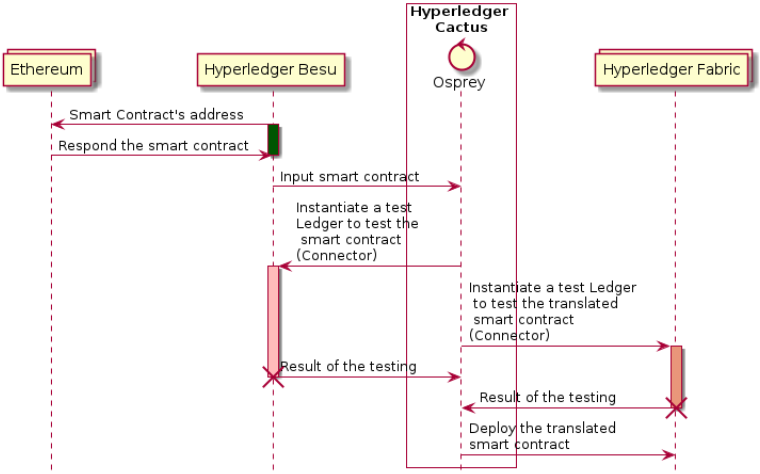
\includegraphics[scale=0.45]{sequence.png}
  \centering
  \caption{Sequence diagram \protect\cite{abrunhosa_2021}}
  \label{fig:sequence}
  \vspace{-2mm}
\end{figure}

Contrarily to the current implementation of Osprey, this solution will implement the inverse of its existing logic. Currently, as discussed in Section \ref{osprey} and as pictured in Figure \ref{fig:sequence}, Osprey takes advantage of Hyperledger Besu to acquire smart contracts from Ethereum and, at the end of the translation process, it deploys them on Fabric. This projects intends to implement the opposite path. That is, contracts are acquired from Hyperledger Fabric and, later, the translated version can be deployed on Ethereum (most likely on a testnet) through Hyperledger Besu. %This means that changes will only take place on the level of the \textit{Migrator Plugin}, referenced on Figure \ref{fig:integration}, and the integration with Hyperledger Cactus will remain unchanged.
Table \ref{table:osprey-comp} summarizes the differences between the current and the future implementations of Osprey.

\begin{table}[]
\centering
\begin{tabular}{ccc}
\hline
Features & \begin{tabular}[c]{@{}c@{}}Current version\\ of Osprey\end{tabular} & \begin{tabular}[c]{@{}c@{}}Future version\\ of Osprey\end{tabular} \\ \hline
Solidity \ding{221} Typescript & \ding{51} & \ding{51} \\
Typescript \ding{221} Solidity & \ding{55} & \ding{51} \\
Translation of other languages & \ding{55} & \ding{55} \\ \hline
\end{tabular}
\vspace{4mm}
\caption{Comparison between versions of Osprey}
\label{table:osprey-comp}
\vspace{-6mm}
\end{table}

%explicar melhor todo o processo
In more detail, the upgraded version of Osprey will be able to receive a smart contract written in Typescript chaincode and parse it into an Abstract Syntax Tree, according to the syntax and rules of the programming language. The \textit{parser} module is responsible for this first task. Then, the AST is properly interpreted by the \textit{converter} module and the solidity smart contract is constructed. The final step consists of testing the behavior of both the original and the translated smart contracts to demonstrate that the target contract kept the original intended behavior. This last stage is performed by the \textit{tester} module. Figure \ref{fig:flow} presents an overview of the aforementioned steps that take place during the translation process of the proposed solution.

%figure
\begin{figure}
  \vspace{-2mm}
  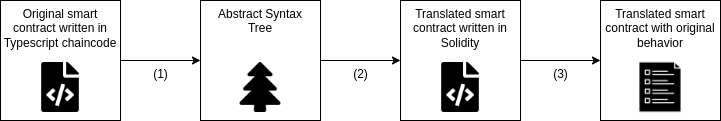
\includegraphics[width=\linewidth]{flow.png}
  \centering
  \caption{Flowchart of the solution}
  \label{fig:flow}
  \vspace{-2mm}
\end{figure}

%explicar 3 fases - translation, testing & deployment
Ultimately, the work flow of the tool can be categorized into three distinct phases: 
\begin{enumerate}
    \item Translation phase;
    \begin{enumerate}
        \item Parsing;
        \item Conversion.
    \end{enumerate}
    \item Testing phase;
    \item Deployment phase.
\end{enumerate}

The first phase is subdivided into two stages that are respectively conducted by the \textit{parser} and \textit{converter} modules. These equate to steps 1 and 2 displayed by Figure \ref{fig:flow}. The parsing stage takes the code of the original smart contract and generates the Abstract Syntax Tree that represents that program. The conversion stage interprets the AST and constructs the target smart contract.

The second phase is accomplished by the \textit{tester} module and is represented by the third step of Figure \ref{fig:flow}. As mentioned before, this phase ensures that the translated code kept the behavior of the original smart contract and executes as intended. This stage is particularly important since it validates if the tool managed to properly translate the original smart contract or not. If not, it means that the tool does not correctly handle a certain type of operation, and improvements and fixes should be applied.

The last phase is optional and consists of allowing the deployment of the translated contract on the target blockchain (i.e., Ethereum mainnet or testnets). This can be achieved because of the integration with Hyperledger Cactus, which provides mechanisms to deploy the translated smart contract on Ethereum through an interaction with Hyperledger Besu. 

% diagrama UML (???)

% talk about how behavior can slightly change and even introduce vulnerabilities
%----------------------------------------------------------------------------- 
\section{Evaluation} \label{evaluation}

After being implemented, the proposed tool should be properly evaluated. This will be done in four different ways:
\begin{itemize}
    % \item By measuring the time it takes for the tool to translate a small set of smart contracts;
    \item By assessing the performance of the migrating tool according to two parameters:
    \begin{enumerate}
        \item Throughput: the amount of smart contracts that can be translated within a unit of time.
        \item Latency: The average time it takes for the tool to translate a smart contract.
    \end{enumerate}
    \item By conducting a survey with a target audience of individuals with knowledge and interest in blockchain technology and smart contract programming about the execution and the output of the tool.
    \item By performing manual verifications to validate the execution and the output of the tool.
    \item By using the tool to translate a Solidity smart contract to Typescript chaincode and then using it again to translate it back to Solidity.
\end{itemize}

The objective of the first approach is to evaluate the performance of the tool, by measuring the average time of translations and the average amount of translations that can be done within a unit of time. Moreover, it may also be possible to reach some conclusions regarding how the complexity of a smart contract and its operations can affect the throughput and the latency of the tool. To do so, a set of smart contracts will be selected from \textit{GitHub} and other online sources to create a dataset suitable to these experiments. %This tests will be executed on a 40 GB RAM machine with an Intel Core i7-11800H CPU and 1 TB SSD of storage. 
The tests that were carried out to evaluate the current version of Osprey show that the tool takes an average of 3.68 milliseconds to translate a fairly simple smart contract. These tests were executed with a dataset of 13 smart contracts that were translated 10000 times \cite{abrunhosa_2021}. Therefore, the future version of Osprey should be evaluated with a dataset of smart contracts of similar complexity and should have a similar performance. This implies that the upgraded version of Osprey should, on average, take about the same time to translate a smart contract (i.e., both measurements should have the same order of magnitude) as the current one.

The second approach will allow to measure the readability of the output of the proposed tool and perhaps help drawing some conclusions regarding a generalized opinion about the utility of the tool and the value it may bring to the ecosystem.

Furthermore, manual verifications can also be important to validate the behavior of the translated smart contract and the appropriate functioning of the tool. This can be specially significant in scenarios where the tool fails to automatically assert the validity of the translated code (i.e., whether or not the target smart contract does what it is expected to do). Such cases can happen in two possible scenarios:
\begin{itemize}
    \item The target smart contract was not properly translated and, in fact, it does not do what was initially intended;
    \item The target smart contract was properly translated but the automatic tests failed to assert that.
\end{itemize}

In such scenarios, resorting to manual validation can help assess what went wrong: the translation process or the testing process. This can be achieved, for instance, through manual deployment of the translated smart contract on the target blockchain and respective execution of its functions. If the execution of the translated code is not aligned with the original behavior of the smart contract, it means that the translation process failed. Otherwise, it indicates that the testing process was miscarried.

Lastly, when converting a Solidity smart contract to Typescript chaincode and then back to Solidity, the final output of the tool should match the original input. In theory, for each Solidity smart contract, the tool should be able to translate it to Typescript chaincode and then translate it back to Solidity, outputting the same code that was originally inputted.


%----------------------------------------------------------------------------- 
\section{Work Schedule} \label{schedule}

This section will go over the work schedule that  that is expected to be conducted during the implementation of the proposed tool. Figure \ref{fig:schedule} presents the estimated time that each planed task of the project will take to be completed throughout the semester.

\begin{figure}
\begin{adjustbox}{max totalsize={\textwidth}{.7\textheight},center}
    \begin{ganttchart}[
        vgrid,
        ]{1}{38}
        \gantttitle{Feb'22}{4} 
        \gantttitle{Mar'22}{5}
        \gantttitle{Apr'22}{4}
        \gantttitle{May'22}{4}
        \gantttitle{Jun'22}{5} 
        \gantttitle{Jul'22}{4} 
        \gantttitle{Aug'22}{5} 
        \gantttitle{Sep'22}{4} 
        \gantttitle{Out'22}{3} \\
        \gantttitlelist{1,...,38}{1} \\
        \ganttbar{(1)}{1}{4} \\
        \ganttbar{(2)}{1}{17} \\
        \ganttbar{(3)}{10}{26} \\
        \ganttbar{(4)}{18}{31} \\
        \ganttbar{(5)}{10}{35} \\
        \ganttbar{(6)}{32}{35} \\
        \ganttbar{(7)}{16}{17}
        \ganttbar{}{25}{26}
        \ganttbar{}{30}{31}
        \ganttbar{}{35}{36} \\
        \ganttbar{(8)}{14}{37} 
    \end{ganttchart}
\end{adjustbox}
Legend: 

(1) - Familiarization with Osprey source code

(2) - Parser implementation

(3) - Converter implementation

(4) - Tester implementation

(5) - Tool review

(6) - Last improvements and fixes

(7) - Tool evaluation

(8) - Writing dissertation

\caption{Planned Work Schedule}
\label{fig:schedule}
\end{figure}

The initial focus of the project will be on the implementation of the parser component that will allow to obtain an Abstract Syntax Tree from the original Typescript chaincode. Then, the implementation of the converter will begin. By integrating this component with the parser, it will be possible to convert the AST into Solidity code. Next, comes the implementation of the tester module that will allow to compare the behavior of both the original and the target smart contracts. In the meantime, the tool should be thoroughly reviewed along the development of each component. Lastly, any last improvements and fixes should be applied and the tool should be properly evaluated based on the defined criteria. When a significant part of the project has already been done, the task of writing the dissertation should begin. This will be the last phase of the project to be finalized.


%----------------------------------------------------------------------------- 
\section{Conclusion} \label{conclusion}
Blockchain interoperability and smart contract migration have become outstanding subjects in blockchain technology. The latter, in particular, can unquestionably help developers once fully implemented and settled in this space. This industry can benefit a lot from it since it can significantly reduce the time of development and allow both developers and enterprises to move across different blockchains or deploy their projects on several platforms at the same time without having to redo previous work (i.e., manually code the same algorithm and applications in other programming languages).

The proposed solution extends an existing tool called Osprey, that is already able to migrate smart contracts from Ethereum to Hyperledger Fabric, by translating Solidity code to Typescript chaincode. By extending this tool to also support smart contract migration from Hyperledger Fabric to Ethereum through translation of Typescript chaincode to Solidity, Osprey will become a full two-way migrating tool. Therefore, enabling developers and enterprises to move between these two platforms in both directions.



%-----------------------------------------------------------------------------
%----------------------------------------------------------------------------- 
%----------------------------------------------------------------------------- 
\newpage




% ---- Bibliography ----
% BibTeX users should specify bibliography style 'splncs04'.
% References will then be sorted and formatted in the correct style.
\bibliographystyle{splncs04}
\bibliography{refs}



\end{document}
